\documentclass[a5paper]{article}

% babel: real Canadian English!
\usepackage[canadian]{babel}
% charter: Bitstream Charter BT font
\usepackage{charter}
% fontenc: encoding for fonts
\usepackage[T1]{fontenc}
% inputenc: source files are in UTF-8. 'ucs' must be loaded first
\usepackage{ucs}
\usepackage[utf8x]{inputenc}
\usepackage{parskip}
  \setlength{\parindent}{18pt}
\usepackage{tikz}
  \usetikzlibrary{positioning}
\usepackage[margin=10mm]{geometry}

\title{Quality of Thought}
\author{DuPont Company\footnote{As provided by D. Colcleugh in \emph{APS501 Leadership \& Leading for Groups \& Organizations}, University of Toronto, 2008. Reset in LaTeX by P.N. Kishimoto \texttt{<pnk@mit.edu>}, 2010.}}
\date{}
\pagestyle{empty}

\begin{document}
\maketitle
\thispagestyle{empty}

\section*{The Components of Thought}
A useful way of starting to think about thinking is to every ``thought'' falling into three componont parts:
\begin{itemize}
  \item its ``level,'' on a scale that we'll look at in a moment.
  \item the ``mental energy'' reflected in it.
  \item the ``modes of behavior'' or values reflected in it.
\end{itemize}
We're going to look at each of these pieces in turn, but you might like to keep this picture in mind as we go: [snip]

% \begin{figure}[h]
% \centering
% \begin{tikzpicture}[every to/.style={draw},every node/.style={pos=0.5,font=\large}]
%   \node[draw,circle,line width=2pt,minimum size=0.8\textwidth] (c) at (0,0) {};
%   \path (c.center) to (c.north) node [anchor=west,text width=7ex,text centered] {Levels of Thought}
%     (c.center) to (c.east) node [anchor=north] {Levels of Energy}
%     (c.center) to (c.south west) node [anchor=south,rotate=45] {Modes of Behaviour};
% \end{tikzpicture}
% \end{figure}

\section{Levels of Thought}
Whenever we have a thought about doing something---anything at all from going to the store to building a better world---the particular thought which we have at any one time can be placed somewhere on this scale:
\begin{itemize} \setlength{\itemsep}{0pt}\setlength{\parskip}{0pt}
  \item \textbf{\scshape Belief}
  \item \textbf{\scshape Philosophy}
  \item \textbf{\scshape Principle}
  \item \textbf{\scshape Concept}
  \item \textbf{\scshape Strategy}
  \item \textbf{\scshape Design}
  \item \textbf{\scshape Action}
  \item \textbf{\scshape Audit}
  \item \textbf{\scshape Evaluate}
\end{itemize}
Let's take a simple illustration.

You are one of a group of friends who enjoy getting together from time to time.
One person normally comes up with an idea for each get-together and organizes it.

You find yourself thinking about these get-togethers.
\begin{itemize}
  \item If your thought is ``It's important to me to spend time with my friends,'' that would be a \textbf{\scshape Belief} about getting together.
  \item If your thought is ``It's very satisfying when we all get together: It keeps our friendship alive and healthy; we trade news and views with people we like and trust; we have fun together''---that's a \textbf{\scshape Philosophy} about getting together.
  \item If your thought is ``When we get together, we always have a program (swimming, skiing, playing ball), we always bring the kids, we keep it simple, we all pitch in to share the cost''---these would be \textbf{\scshape Principles} (or standards) about get-togethers.
  \item If your thought is ``I'll organize a get-together for next weekend in my backyard.
    We'll all enjoy a swim in the pool and a barbecue while the weather is still good''---that would be a \textbf{\scshape Concept} for a get-together.
  \item If your thought is ``I'll have to figure out a whole bunch of things that will have to be done if I'm going to get something organized''---things like:
    \begin{itemize}
      \item invitations
      \item mow the lawn
      \item clean the pool
      \item borrow some chairs and a second barbecue
      \item etc., etc.
    \end{itemize}
    you would be at the \textbf{\scshape Strategy} level of thought about a get-together.
  \item If your thought is ``Now, I'd better get ways and means of doing these things figured out and put down on a piece of paper'':
    \begin{itemize}
      \item First, get Bill to phone everybody
      \item Next, ask John and Sue to line up a dozen chairs and bring them over on Saturday morning
      \item Next, get the neighbour's kid lined up to mow the lawn on Friday
      \item etc., etc.
    \end{itemize}
    you would be at the \textbf{\scshape Design} level of thought about a get-together.
  \item If your thought is ``I'm going to start right now'' and you reached for the phone, you would be at the \textbf{\scshape Action} level of thought about the get-together.
  \item If, as the day of the get-together got closer, you kept thinking about how everything was coming along and fitting together---you'd be at the \textbf{\scshape Auditing} level of thought about the get-together.
  \item If, during the get-together, you kept checking how things were going---was it time to eat?
    Did everybody have something to drink?
    Was everybody getting involved and having fun?
   ---you would be at the \textbf{\scshape Evaluating} level of thought about the get-together.
\end{itemize}
Now, the point about that example is not that everybody's mind works that way, in a neat and tidy flow from top to bottom.
It doesn't!

And it's not an argument that everybody's mind should work that·way, all of the time.
We'd never get anything done!

What it is, first of all, is an illustration of the many different ``levels of thought'' we can be at when we're thinking about something, and how each ``level'' of thought is different.

Next, it's an illustration of how these different levels of thought are in fact inter-connected and tied together, even if we haven't consciously recognized it before.
\begin{itemize}
  \item Our \textbf{\scshape Beliefs} lead to our \textbf{\scshape Philosophy} and it leads to the \textbf{\scshape Principles} we follow.
  \item Together they answer the question of ``why'' we think something---or want to create or do something (and don't think of doing something
different)---at particular points in time.
  \item Once we have thought out why we want to do something, we can develop a \textbf{\scshape Concept} (or idea) of what it is and what it would look like, and then we can develop our overall \textbf{\scshape Strategy} for getting it done and for bringing the result into existence; and we can then \textbf{\scshape Design} a specific set of ways and means for doing so.

    These show us ``how'' to think about creating the result we want.
  \item With this in hand, we can begin to take \textbf{\scshape Action}, and \textbf{\scshape Audit} and \textbf{\scshape Evaluate} our action in a systematic way as we move along.
  \item These are the ``what'' steps in getting something done, in creating something.
\end{itemize}
\begin{figure}[h]
\centering
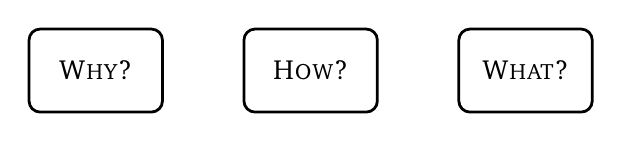
\begin{tikzpicture}[every to/.style={draw,->,line width=1pt,shorten >=2pt},every node/.style={draw,line width=1pt,rounded corners,minimum height=3em,minimum width=10ex,font=\scshape}]
  \node (a) {Why?};
  \node (b) [right=1cm of a.east] {How?};
  \node (c) [right=1cm of b.east] {What?};
  \path (a) to (b); \path (b) to (c);
\end{tikzpicture}
\end{figure}

When we can answer the question ``Why am I thinking of doing this?'' to our own satisfaction; and can answer the question ``How am I going to do it'' in a way that takes everything that needs to be thought about into account: and can then answer the question ``What am I going to do?'' in a systematic way---then we are using all the levels of thought in a conscious, organized and disciplined way that is most likely to get the creative and satisfying results we want.

What we have talked about so far can be summarized as follows:



Being conscious of levels of thought is helpful and useful in a variety of ways:
\begin{itemize}
  \item overall, as we have seen, it gives us a framework for seeing a total flow or network of related thoughts about something
  \item at any moment, the list gives us the ability to ``locate'' a thought we are having, and to describe what it is and where it is more clearly than we could do before:
    \begin{itemize}
      \item I'm down at \textbf{\scshape Design}
      \item I'm still up at \textbf{\scshape Principle}
    \end{itemize}
  \item this ability to ``locate'' and ``describe'' our thoughts gives us a chance to check the consistency and flow of our own thinking:
    \begin{itemize}
      \item If I'm now working on \textbf{\scshape Design}, what \textbf{\scshape Concept} is it I'm trying to put.in place?
      \item If I'm in \textbf{\scshape Action}, can I remember what I \textbf{\scshape Principles} I was trying to follow?
    \end{itemize}
  \item this, in turn, gives us a way to test and connect our thinking:
    \begin{itemize}
      \item If, when we're thinking about \textbf{\scshape Design}, we just can't seem to get it to come out right, we can consciously and systematically work backwards, through \textbf{\scshape Strategy}, \textbf{\scshape Concept}---all the way back to \textbf{\scshape Belief} if necessary---to see whether we missed something, or skipped something, or need to clarify something at an upper level, before we can go forward effectively.
    \end{itemize}
\end{itemize}
All levels of thought are needed and can be useful in particular situations.
There is no good or bad level of thought.

Finally, there is another very important---valuable---use for levels of thought.
If all of us understand them in the same way, and use the same name for each of the levels, then our ability to share our thoughts with others will improve enormously:
\begin{itemize}
  \item If I say to you---``I'm thinking of such-and-such a subject, and I'm trying to develop a \textbf{\scshape Concept}'', you now know immediately where I am and what I mean.
  \item If, as happens more often, I just start talking about such-and-such in a muddled or confused way, you can stop me and say ``Just a minute! I don't understand where you are on this thing---are we talking \textbf{\scshape Beliefs} or \textbf{\scshape Principles} or \textbf{\scshape Concept} or what?
    Where does your thinking stand on these?''
  \item If someone comes to you and lays out a proposal to do something, levels of thought is an excellent framework to keep in your head as the proposal unfolds!
    \begin{itemize}
      \item Do the various stages of \textbf{\scshape Why}---\textbf{\scshape How}---\textbf{\scshape What} flow in a clear and logical way?
      \item Do they reflect central \textbf{\scshape Beliefs}, \textbf{\scshape Philosophy} and \textbf{\scshape Principles} that you share?
      \item Does the \textbf{\scshape Concept} flow smoothly from the \textbf{\scshape Principles}, and do the \textbf{\scshape Strategy} and \textbf{\scshape Design} fit nicely together?
      \item Are all the elements considered and accounted for? -
      \item Is the \textbf{\scshape Action} a good extension of the \textbf{\scshape Design} and is there proper allowance for \textbf{\scshape Audit} and \textbf{\scshape Evaluating}?
    \end{itemize}
\end{itemize}
If the answer to these questions is ``\textbf{\scshape Yes},'' you may quickly agree with the proposal.
If not, you can use levels of thought to get back to where you need to be to resolve your differences.

This is a disciplined and orderly process---you avoid getting into unnecessary and often heated arguments about detail by focussing on basic levels of thought, where the chance of reaching common agreement is greatest.
\begin{itemize}
  \item If two or more of us are working together on some question or problem, levels of thought is a useful way of thinking about how to tackle the task in a disciplined and productive way instead of rushing down to the \textbf{\scshape Design} or \textbf{\scshape Action} level as we often do, inside the first 10 seconds, and trading interesting but often unconnected or irrelevant thoughts---``Let's do this''. ``No---let's do that''---that often lead nowhere.
\end{itemize}
So much---at this stage---about levels of thought.

Have you been testing this against your own experience?
Trying it out on something you were involved in recently?
Does it give you any ideas you want to pursue?

Are you ready to go on to the next component of thought? `

\section{Levels of Energy}
The second component of thought is ``levels of energy''---the different kinds or levels of mental energy we can find reflected in every thought that we have---and that others have.

The different kinds or levels of mental energy we can identify are:
\begin{itemize}
  \item \textbf{\scshape Automatic}
  \item \textbf{\scshape Sensitive}
  \item \textbf{\scshape Conscious}
  \item \textbf{\scshape Creative}
  \item \textbf{\scshape Unitive}
  \item \textbf{\scshape Transcendent}
\end{itemize}
and I''ll define more closely what these names mean as we go along.

It's a little difficult to describe or define abstractly exactly what is meant by ``mental energy''.

In part, it's a description of the feeling---the emotion, if you want to call it that---which is associated with a particular thought we have, at a particular moment.
How do we ``feel about'' what we're thinking?
What level of feeling do we put into it?
Are we ``turned on'' or ``off''?

In part, mental energy is comparable to the physical energy we can see in different actions we take at different times---sometime low-level, just coasting; other times, quite alert and active; still other times, really
moving and shaking!

Why don't we look at each level of mental energy, and let you consider them for yourself?

Here are descriptions of the different levels:
\begin{description}
 \item[\scshape Automatic] We're scarcely aware that we are thinking at all.
    What we are doing doesn't (or doesn't seem) to require any particular kind of active thought:
    \begin{itemize}
      \item riding the bus
      \item eating lunch
      \item doing any other routine, repetitive, familiar task
    \end{itemize}
  \item[\scshape Sensitve] We know we're thinking.
    We have a reasen for what we are doing.
    We're looking for relationships/differences between things at quite a simple level.
    \begin{itemize}
      \item checking a 6/49 ticket against the numbers in the paper
      \item searching for two matching buttons in a box ef 50 different shapes and sizes.
    \end{itemize}
  \item[\scshape Conscious] We know we're thinking---we're aware of ``why'' we're thinking, what our purpose is.
    We're consciously trying to choose thoughts/ideas/actions that fit a defined purpose:
    \begin{itemize}
      \item trying to figure out when to leave home to pick up two friends and get downtown for the ballgame on time in heavy traffic.
    \end{itemize}
  \item[\scshape Creative] We are consciously and actively thinking about new ideas---new solutiens---new approaches to what we're trying to achieve.
    We are conscious of our own thought processes and we are not satisfied with the ideas we are producing.
    We're pushing our thinking further and deeper to reach a better answer.
  \item[\scshape Unitive] We are trying to get all our thoughts, ideas, means and methods ``lined up'' in a disciplined way.
    We're conscious of the others involved in what we're doing, and we're trying to work out a ``consensus'' that everyone can support.
  \item[\scshape Transcendent] Our thoughts and actions are completely tied-in with those of others, towards a common purpose or goal.
    We are conscious of out own thought processes and those of others, and our thoughts and actions are focussed on finding the best possible solution to what we are working on, regardless of self-interest or past practice, in a way that generates enthusiasm and energy in everyone involved.
\end{description}

Now, if your first reaction is that much of this is hard to grasp, I don't blame you.
Some of these distinctions seem to be a little narrow when you first look at them.
What's the point?

Why don't you go back and read the first descsiption again (\textbf{\scshape Automatic}), and than compare it with the last one (\textbf{\scshape Transcendent}).
I don't think you will have much difficulty in recognizing a vast difference between the ``feeling'' or ``energy'' reflected in these two extremes, or imagining the equally vast differences in thought and behaviour produced at either extreme of ``energy.''

If that is a correct assumption, then you are much more than half way to grasping all you need to understand about ``levels of energy.''
\begin{itemize}
  \item there are big differences in ``energy'' between the two ends of the scale.
  \item these differences in ``energy'' can be expected to have powerfully different effects on ``quality of thought,'' depending on the situation.
\end{itemize}
Note that last phrase, however: ``depending on the situation.''

We all need, and should learn to use, all the levels of energy.
Each one has its place and none of them is good or bad by itself.
What's important, however, is using the appropriate one at the apptopriate time.
\begin{itemize}
  \item \textbf{\scshape Automatic} is a perfectly appropriate level of mental energy to use for taking a shower, particularly if you are using your time under the shower to be \textbf{\scshape Creative} about your plans for the rest of the day.
    The other way around would be quite inappropriate.
  \item You may need to be \textbf{\scshape Unitive} or even \textbf{\scshape Transcendent} when you're running the PTA meeting tonight, but \textbf{\scshape Conscious} is probably more than appropriate when you are ordering a quick sandwich and coffee before you go to the meeting.
    Again, the other way around would be downright foolish and wasteful.
\end{itemize}
It is possible---in words---to split up the difference between the two ends of the mental energy scale into various levels, each one of which moves part way to close the gap.
And that's all the specific descriptions are---steps up the scale of ``energy'' from \textbf{\scshape Automatic} to \textbf{\scshape Transcendent}.

You can go back later, if you want, and trace the steps out for yourself, and see how each one of the descriptions builds on the one before, but falls short of the next one up.

But, you don't have to do so to understand the basic idea of levels of mental energy---and you certainly don't have to memorize each of the descriptions!

\subsection{Using Levels of Energy}
Once you have understood the basic idea behind levels of energy, however, what you are going to have to do is think about how---and when---you can use this understanding and its implications for quality of thought:
\begin{itemize}
  \item How can you practice recognizing differences in your own mental energy from time to time, situation by situation?
  \item How can you go about deciding if you are using the appropriate level of mental energy in each situation?
  \item If you decide you are not, how can you practice, and become skilled at, shifting your level of mental energy from one level to a more appropriate
 one, depending on the situation?
  \item How can you learn to recognize other people's level of energy, situation by situation? What---if anything---can you do to shift other people's energy to a more appropriate level in a given situation?
\end{itemize}

Most of these questions can't be answered in a general way.
Most of the answers depend on you, and on how interested and curious you are.

If this discussion has opened your mind up to questions you haven't thought about before or thrown new light on old questions, and if you are sufficiently curious about yourself and how your mind works, then you will chew away at these questions until you find answers that satisfy you.
Just asking yourself the questions may be enough to get your mind rolling towards answers!
Use the various definitions as a check-list to help you think about and
learn how to identify two things:
\begin{itemize}
  \item What's the situation?
    What level of energy would seem to be most appropriate?
  \item What level am I at right now?
    Is it where I want to be?
\end{itemize}
As you work at these two questions, you'll find the answers moving back and forward between them, until you feel comfortable with both.

The only really useful knowledge is knowledge you acquire for yourself or about yourself, so give it a try!
Put the appropriate ``mental energy'' into it!

We will come back, shortly, to the question about recognizing---and shifting---other people's level of mental energy.

Meanwhile, let‘s move ahead to the third component of thought.

\section{Modes of Behaviour}
The third component of thought is something we can call ``modes of behaviour.''
There are three basic ``modes of behaviour'' which we can find reflected in every thought we have---and in every thought other people have.
These three modes are:
\begin{itemize}
  \item \textbf{\scshape Reactive}
  \item \textbf{\scshape Ego}
  \item \textbf{\scshape Purposeful}
\end{itemize}
When we use the word ``behaviour'' most of us think of actions---what we do or what someone else does is ``behaviour.''
And that is; of course, quite accurate, as far as it goes.

Behaviour---what we do (or don't do) at a point in time---reflects what we are thinking at that moment, however, and it is for this reason that we want to discuss ``modes of behaviour'' as part of quality of thought.

And there is another reason, equally important: what we think, and the modes of behaviour we employ in our thinking and in our actions, show the values we are holding---or that we are applying---at that moment (whether consciously or unconsciously).
Values are totally ``internal'' or mental.

Let's look, then, at the three modes of behaviour and the values they disclose.

First---what do we mean by a ``value''?

For our purposes here, I think the most useful basic description is this---a value is the expression of a principle or standard considered important in life.

Some ``values'' are widely held and often put into words:
\begin{itemize}
  \item honesty
  \item openness
  \item respect for human life
\end{itemize}
There are many other ``values,'' however, which are even more widely held but are deeper and less often identified or put into words: They include such things as:
\begin{itemize}
  \item self-protection
  \item self-assertiveness
  \item success
  \item fulfilment
  \item hope
  \item joy
\end{itemize}
Still other ``values'' are more personal to specific individuals:
\begin{itemize}
  \item Sue values her privacy
  \item John values his family
  \item and so on
\end{itemize}
Values are the expression of principles or standards considered important in life---values are basic to defining who we are and how we think and behave.

At any particular moment, then, in any given situation, our thoughts and our actions exhibit the values we are expressing at that moment.
What is exhibited is the particular value, or set of related values that we consider important at that moment, in that situation.
Our \textbf{\scshape Situational} values.

Which brings us back to ``modes of behaviour.''
By ``modes of behaviour'' I mean, quite simply, the three broad classes or patterns of behaviour (\textbf{\scshape Reactive}, \textbf{\scshape Ego}, \textbf{\scshape Purposeful}) I listed at the beginning---each of which exhibits a certain set of values which the person behaving in each of these modes considers important to apply at that moment, in that situation.

What we see---when we look at ourselves or another person---is behaviour: patterns or modes of thought and behaviour.
What's behind these ``behaviours'' are particular values.
\begin{itemize}
  \item The \textbf{\scshape Reactive} mode describes how we think and behave in response to the environment we are in---including the other people.in that environment.
  \item The \textbf{\scshape Ego} mode describes how we think and behave to achieve our personal aims or goals.
  \item The \textbf{\scshape Purposeful} mode describes how we behave in regard to some (larger) purpose beyond just ourselves.
\end{itemize}
I think it would be fair to say that all of us go into the \textbf{\scshape Reactive} mode when we experience something new---or different, or unusual---for the first time.
We look and listen---we may taste it or smell it---but we do so cautiously.
We hold back from it.
We're on our guard.
We may well be suspicious, even anxious.
What's this all about?
What's going on here?
Will it attack me?

Then, as we gain more experience with whatever it is, as we become more familiar and comfortable with it, we often move on to the second mode---\textbf{\scshape Ego}.
There, we can often find a personally useful or relevant may to use the new thing, the new situation, to our personal advantage.
We use it, in ways that make sense to us, that have a payoff, for us.

Then, as we use it and derive benefit or advantage from it, we may move to the third mode---\textbf{\scshape Purposeful}.
We may begin to see not just a way for whatever-it-is to be of use or advantage to us personally, but a way for it to be useful or usable in achieving something in a larger context.
We extend our thinking about whatever-it-is beyond ourselves and our own
 self-interest and immediate needs.

Let's take an example.

Not too many years ago, Personal Computers didn't exist, and few of us knew much about any kind of computers.
We got funny cards with our phone bills and computer printouts crossed our desks, but keyboards, discs, drives, programs, storage and chips were just distant jargon.

Then, computers got closer---and closer.
We began to hear about word processors, remote terminals, personal, even portable, computers.
Then one showed up down the hall.
Then another.

How did we behave?
We were \textbf{\scshape Reactive} at first.
What's this?
What's it going to do to me?
What does it do, anyway?
How does it work?
You mean I'm going to have to learn that?
Some ``reactions'' were even stronger---No way!
Not me!

But time moved on.
And then the Company offered to subsidize the purchase of PC's by employees for personal use.
What happened?
Over 500 were snapped up!
These 500 people had moved from \textbf{\scshape Reactive} to \textbf{\scshape Ego} so far as computers were concerned!
They had seen ways to use a PC to pursue their personal purposes and interests.

Inside the Company, too, a similar behaviour swing could be observed in many people as they became more familiar with word processors and terminals.

What happened next?

Soon stories started flowing back along these lines---``I bought it to play with, to do my income tax, etc. and before you knew it all of as were using it---my husband, my wife, the kids.
We've found dozens of ways to use it that make sense ---
We're looking for new programs all the time.''

And, then, ideas for at-work applications began flowing in---``Why don't we give all the sales reps. a portable---why don't we try others---why don't we try that---use one for this ---''

What was happening was a second switch, from \textbf{\scshape Ego} to \textbf{\scshape Purposeful} thinking and behaviour, with respect to computers, on the part of many people.

\begin{figure}[h]
\centering
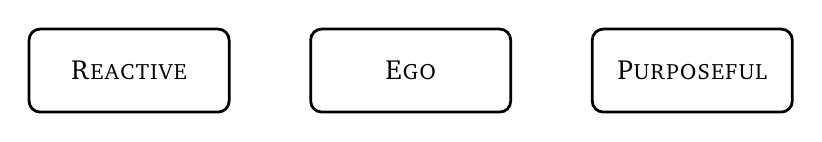
\begin{tikzpicture}[every to/.style={draw,->,line width=1pt,shorten >=2pt},every node/.style={draw,line width=1pt,rounded corners,minimum height=3em,minimum width=15ex,font=\scshape}]
  \node (r) {Reactive};
  \node (e) [right=1cm of r.east] { Ego};
  \node (p) [right=1cm of e.east] { Purposeful};
  \path (r) to (e); \path (e) to (p);
\end{tikzpicture}
\end{figure}

Each mode of behaviour was appropriate at the time it occurred, and demonstrated the specific values people were applying at that time, combined with their state of knowledge, familiarity and comfort with the idea of computers.

What happened, over time, was not a change in people's overall values---what happened was that, as the situation changed, the specific values which people expressed or exhibited in their behaviour changed.
Their \textbf{\scshape Situational} values changed as their understanding of the \textbf{\scshape Situation} changed.

What does all of this mean for us?
What does it do to help us understand---and improve---our quality of thought?

When we think about the profound differences between the extremes of modes of behaviour---from \textbf{\scshape Reactive} to \textbf{\scshape Purposeful}---we begin to recognize how much our own thinking, moment by moment, must be ``colored'' by our own immediate and particular mode of behaviour and by our situational values.

Do new ideas, new situations, new people to deal with---do those things make you \textbf{\scshape Reactive}?
How cautiously do you approach them?
Do you approach them at all---or are you so \textbf{\scshape Reactive} you avoid them---pretend they don't exist?
Do you stubbornly protect the status quo?
Turn off?

Where, and when, do you feel in the \textbf{\scshape Ego} mode?
How did you get there?
Did it just happen, or did you have to work at it?
What turned you on?
Did you notice the difference?
Did it make you feel good?

How about \textbf{\scshape Purposeful}?
Are you involved in situations (other than work) that take you beyond yourself---clubs, school committees, local affairs, politics?
How do you ``behave'' when that's what you are doing?
What do you look at?
Think about?
How did you learn to do that?

All of these questions are ways of going about answering the fundamental questions for yourself.
Only you know yourself well enough to puzzle it out.
And you can---and will, for ``modes of behaviour'' are too basic for you to ignore for long.

There are all kinds of perfectly reasonable and natural explanations for this, and these need not concern us here.
What we need to remember is simple and easy to state:
\begin{itemize}
  \item none of us ``sees'' everything there is to see in a situation.
  \item each of us probably ``sees'' quite different things---different slices of the situation.
  \item we can be aware of these facts, and we can do many things to train ourselves to ``see'' more completely and more accurately, but no matter how hard we try it's impossible to ``see'' everything.
  \item if you are trying to understand a complex situation, therefore, it may not be very useful just to think about what you ``saw''---you could get a fuller and clearer ``view'' of the situation if you added various people's ``views'' together.
    The situation might look very different to you then.
    You might understand it a great deal better.
    (Do you remember the story of the blind men and the elephant?)
    If you understood it better---more completely---you would be able to think more effectively about it.
\end{itemize}
What you see is what you get: what you get is what you see!
Whichever way you want to phrase it, it's true.

Beware then: Learning to think effectively about the things that we sense is only part of the story: We must also think about---and do something about---the quality and completeness of what we sense, of our inputs, of the raw material of many of our thoughts.

\section*{Mental Processes}
We all use a range of mental processes:
\begin{itemize}
  \item We have ways of ``sensing'' what is going on in the world around us;
  \item We have ways of evaluating---sizing up---what our senses bring us;
  \item We have ways of picking through what we have sensed, and making patterns out of it that are useful or interesting to us;
  \item And we have ways of setting objectives for ourselves, of deciding goals and priorities.
\end{itemize}
We're not going to talk of all of these now: The one we need to spend a few minutes·on right now is ``sensing''.

All the data we have about the world ''out there'' comes to us through our senses.
Agreed?
Of course!

But---did you ever stop to consider how selectively most of us use our senses?
Three people could walk together down a country road.
After 30 minutes:
\begin{itemize}
  \item the bird watcher could give you a detailed list of the 15--20 species he had seen.
  \item the wildeflower fancier could tell you all about the rich assortment he had seen and identified by the roadside.
  \item the woodsman could name every kind of tree he had seen and the age and condition of each.
  \item none could comment usefully on what the others reported---they would claim they ``hadn't seen'' these other things!
\end{itemize}

Sound familiar?
A bit exaggerated, perhaps, but exaggerated only to make the point: For a whole variety of reasons, none of us ever sees everything there is to see in a-situation---and what we think we see is often only a very small slice of reality.
\end{document}
